\documentclass{whutmod}
\usepackage[linesnumbered,ruled,lined]{algorithm2e}
\bibliographystyle{unsrt}
\team{10}
\membera{刘子川}
\joba{编程}
\memberb{程宇}
\jobb{建模}
\memberc{祁成}
\jobc{写作}
\hypersetup{
	colorlinks=true,
	linkcolor=black,citecolor=black
}


\newcommand{\upcite}[1]{\textsuperscript{\cite{#1}}}
%%%%%%%%%%%%%%%%%%%%%%%%%%%%%%%%%题目%%%%%%%%%%%%%%%%%%%%%%%%%%%%%%%%%%%%
\title{基于xxxxxxxx模型}
\tihao{3} 

\everymath{\displaystyle}

\begin{document}

	\maketitle
	\thispagestyle{empty}
%%%%%%%%%%%%%%%%%%%%%%%%%%%%%%%%%摘要%%%%%%%%%%%%%%%%%%%%%%%%%%%%%%%%%%%%
	\begin{abstract}
		控制高压油管的压力变化对减小燃油量偏差,提高发动机工作效率具有重要意义。本文建立了基于质量守恒定理的微分方程稳压模型,采用二分法、试探法以及自适应权重的蝙蝠算法对模型进行求解。
		//
	
		针对问题一,建立基于质量守恒定律的燃油流动模型,考察单向阀开启时间对压力稳定性的影响。综合考虑压力与弹性模量、密度之间的关系,提出燃油压力-密度微分方程模型和燃油流动方程。本文采用改进的欧拉方法对燃油压力-密度微分方程求得数值解;利用二分法求解压力分布。综合考虑平均绝对偏差等反映压力稳定程度的统计量,求得直接稳定于100MPa的开启时长为\textbf{0.2955ms} ,在2s、5s内到达并稳定于150MPa时开启时长为\textbf{0.7795ms}、\textbf{0.6734ms},10s到达并稳定于150MPa的开启时长存在多解。最后对求解结果进行灵敏度分析、误差分析。
		//
	
		针对问题二,建立基于质量守恒定律的泵-管-嘴系统动态稳压模型,将燃油进入和喷出的过程动态化处理。考虑柱塞和针阀升程的动态变动,建立喷油嘴流量方程和质量守恒方程。为提高角速度求解精度,以凸轮转动角度为固定步长,转动时间变动步长,采用试探法粗略搜索与二分法精细搜索的方法求解,求得凸轮最优转动角速度\textbf{0.0283rad/ms(转速270.382转/分钟)},并得到该角速度下高压油管的密度、压力周期性变化图。对求解结果进行误差分析与灵敏度分析,考察柱塞腔残余容积变动对高压油管压力稳态的影响。
		//
	
		针对问题三,对于增加一个喷油嘴的情况,改变质量守恒方程并沿用问题二的模型调整供、喷油策略,得到最优凸轮转动角速度为\textbf{0.0522rad/ms(498.726转/分钟)};对于既增加喷油嘴又增加减压阀的情况,建立基于自适应权重的蝙蝠算法的多变量优化模型,以凸轮转动角速度、减压阀开启时长和关闭时长为参数,平均绝对偏差MAD为目标,在泵-管-嘴系统动态稳压模型的基础上进行求解,得到最优参数:\textbf{角速度0.0648 rad/ms(619.109转/分钟)}、减压阀的开启时长\textbf{2.4ms}和减压阀的关闭时长\textbf{97.6ms}。
		//
	
		本文的优点为:1. 采用试探法粗略搜索与二分法精细搜索结合的方法,降低了问题的求解难度。2.以凸轮转动角度为固定步长,对不同角速度按照不同精度的时间步长求解,大大提高了求解的精确度。 3.针对智能算法求解精度方面,采用改进的蝙蝠算法,使速度权重系数自适应调整,兼顾局部搜索与全局搜索能力。
		
		\keywords{
			微分方程\quad
			微分方程\quad	
			微分方程\quad
			微分方程\quad
		}
	\end{abstract}


%%%%%%%%%%%%%%%%%%%%%%%%%%%%%%%%%目录%%%%%%%%%%%%%%%%%%%%%%%%%%%%%%%%%%%%
	\thispagestyle{empty}
	\tableofcontents
	\setcounter{page}{0}                                               
	\newpage	%换页符
	

	
	\section{问题重述}	
		\subsection{问题背景}
	    	由部署在监控区域的大量低成本微传感器节点组成的网络系统,称为无线传感器网络(Wireless Sensor Network,WSN)。WSN 节点通过无线信道相互通信,协同感知,收集和处理监控区域内传感对象的信息,然
	    	后将信息发送给观察者\upcite{1}。因此,WSN广泛应用于自然灾害预警,环境监测,战场监视等领域\upcite{2}。
	    	能源对无线传感器网络的发展至关重要。传感器节点通常由装载电池或超级电容器供电,但由于传感器节点尺寸较小,装载的电池容量有限,有时因为维护成本过高而无法延长无线传感器网络的生命周期,这限制了无线传感器网络的发展和应用。前人采用能量平衡\upcite{4,5},移动传感器\upcite{6,7}和移动收集器等方案来节省能量从而达到延长网络生命周期的目的。然而,这些方案仅降低能量消耗率,不能真正延长WSN 的生命周期。

	    	
	    	而在按需充电结构的无线可充电传感器网络(Wireless Rechargeable Sensor Network,WRSN)中,节点主动监视其自身的剩余能量,当其能量水平低于某个阈值时,向BS发送充电请求。BS 根据某些充电规则对请求节点建立充电调度队列,并将该调度发送给 WCD 从而引导WCD 为节点进行充电服务\upcite{3},如图\ref{lasbel}所示。传统的调度方案只考虑时间,空间或两者混合因素。由于受到空间、时间和能量因素的制约,传统的调度方案仅能满足少量的充电请求节点,这导致 WRSN 在繁忙的网络环境中生命周期比较短\upcite{3}。为了减小移动充电器在路上的能量消耗,需要合理地规划移动充电器的充电路线。
				\begin{figure}[H]
		\centering
		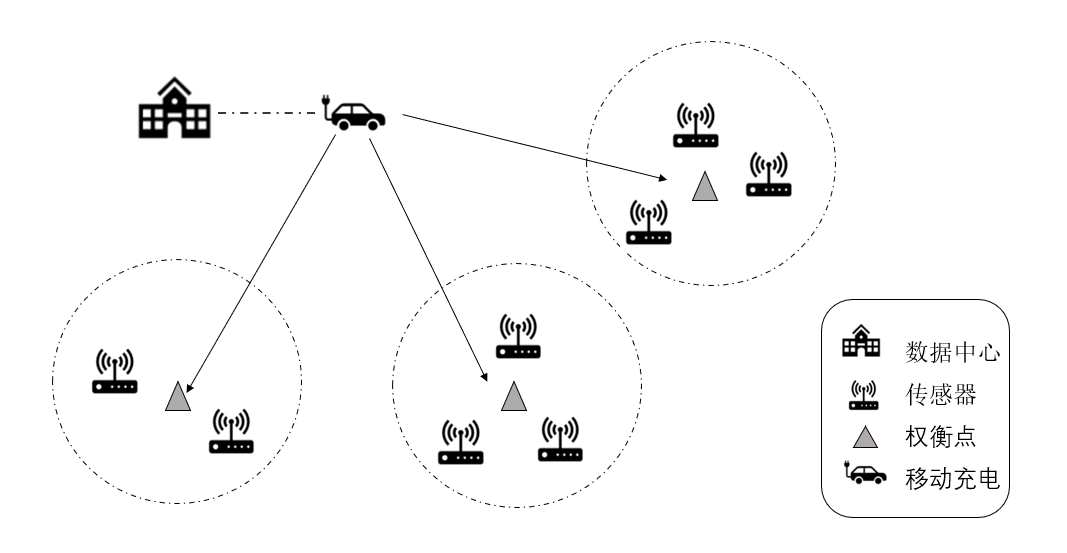
\includegraphics[width=\textwidth]{figures/demo.png}
		\caption{无线可充电传感器网络架构示意图}\label{lasbel}
	\end{figure}
	
		\subsection{问题概述}
		    围绕相关附件和条件要求,研究一个或多个移动充电器在各传感器间的充电路线方案,依次提出以下问题:
				 
			
			\textbf{问题一:}当只派出一个移动充电器时,如何规划移动充电器的充电路线才能最小化移动充电器在路上的能量消耗。
			
			\textbf{问题二:}在只派出一个移动充电器的情况下,若采用问题一中规划出来的充电路线,每个传感器的电池的容量应至少是多大才能保证整个系统一直正常运行?
			
			\textbf{问题三:}为了提高充电效率,同时派出4个移动充电器进行充电,在这种情况下应该如何规划移动充电器的充电路线以最小化所有移动充电器在路上的总的能量消耗?每个传感器的电池的容量应至少是多大才能保证整个系统一直正常运行?

	
	\section{模型假设}

		\begin{itemize}  
				\item [(1)] 假设充电场景不属于时变充电方案,即传感器解节点充电时单位时间的收发数据能量不随时间改变而改变。
		\item [(2)] 考虑移动充电器MC可以同时为多个节点进行无线充电,即其具有一定的充电范围,并且在此范围内充电场的能级不随距离而发生变化。                 
		\item [(3)] 由于传感器分布区域较小,本文忽略地球曲率的影响,即假设所有传感器分布在同一个二维平面上。
		\item [(4)] 假设小车在移动时的能量消耗功率为恒定值,即其不随移动路段和工作时间而改变。

		\end{itemize}

		
	\section{符号说明}
		\begin{table}[H]
		\centering
		\setlength{\tabcolsep}{12mm}
		\begin{tabular}{cc}
			\toprule[1.5pt]
			\multicolumn{1}{m{5cm}}{\centering 符号} & \multicolumn{1}{m{5cm}}{\centering 说明} \\
			\midrule[1pt]		
			$P_n$  & 20个站点  \\ 
			$P_n$  & 20个站点  \\ 
		   	$P_n$  & 20个站点  \\ 
			\bottomrule[1.5pt]
		\end{tabular}
		\begin{tablenotes}
		\item 注:表中未说明的符号以首次出现处为准
		\end{tablenotes}
		\end{table}

	\section{问题一模型的建立与求解}
		\subsection{问题描述与分析}

%			问题一要求充电路线最小化移动充电器在路上的能量消耗。在周期性场景中,均以最大化驻站空闲时间比为目标,移动充电设备均从服务站(即维护站)出发,完成充电活动后回到服务站。Kurs等人\upcite{4}最先提出对网络中所有节点进行固定周期T的遍历充电模型。移动无线充电设备(Wireless Charging Vehicle, WCV)从服务站出发,依次为网络中所有节点进行点对点的无线充电,最终又回到服务站。
%			
%			根据无线传感器网络模型,每个固定位置的基站传感器节点具有通信圆域,其半径为$R$,无线充电设备在通信圆域内以固定速率$r$充电,
%
%		\subsection{模型的求解}
		
			问题一要求充电路线最小化移动充电器在路上的能量消耗。为使得无线传感器网络
		(Wireless Sensor Network,	WSN)持续不断地运行,移动充电器(Mobile Charger,MC)必须在WSN的每一个生命周期中访问所有的传感器节点并对其完成充电并返回数据中心。要使得MC在路上的能量消耗最小,即使得每个周期内MC移动的路程达到最小,当MC为传统的短程有线充电设备时,该问题可被转化为传统的TSP问题。
		    
		    分析整理相关文献可知(引用),随近代无线充电技术发展,WSN的充电任务将由负载无线充电设备的移动充电器(Wireless Charging Vehicle,WCV)完成。WCV可在距离目标传感器一定范围内对其执行无线充电,且可同时对多个传感器进行无线充电,假设在此范围内充电场的能级不随距离而发生变化,并尝试优化求解在充电设备的最大充电距离为不同值时的最佳充电路线。
		    
		    本节首先使MC为传统的短途有线充电设备,使得可充电距离$R=0$,即将问题转化为传统TSP优化模型,使用生命遗传算法进行优化求解。之后将MC视为无线充电设备,首先使得$0<R<\frac{\alpha }{2}$($\alpha$表示所有传感器间的距离中的最小值 ),该情况下,MC在任意时刻最多只能对一个传感器进行充电,我们将梯度下降算法嵌入???遗传算法对该情况下的充电路径进行优化求解;当$R\geqslant \frac{\alpha }{2}$,即MC可对多个传感器同时进行充电,针对此情况我们修改???遗传算法的编码方式,即合并可充电区域重叠的传感器编码,求解最佳充电路径。
			
			
			%在周期性场景中,均以最大化驻站空闲时间比为目标,移动充电设备均从服务站(即维护站)出发,完成充电活动后回到服务站。Kurs等人\upcite{4}最先提出对网络中所有节点进行固定周期T的遍历充电模型。移动无线充电设备(Wireless Charging Vehicle, WCV)从服务站出发,依次为网络中所有节点进行点对点的无线充电,最终又回到服务站。
		
		
		
		\subsection{模型的建立}
			\subsubsection{有线充电设备模型}
		    定义传感器坐标点集为$S=\left \{ s_k| 1\leqslant k \leqslant 29,i\in Z\right \}$,其中$s_k$表示附件中的第$k$号传感器对应的坐标位置。当MC为短程有线充电设备时,即充电有效距离$R=0$时,问题一可转化为传统TSP问题。假设MC在移动时的能量消耗功率为定值,为使得其在路上的能量消耗最小,即使得其在每个周期内移动总路程达到最小值。MC的充电路线可表示为二维有限序列如下
		    \begin{gather}
		    P=[ p_{1},\cdots,p_{i},\cdots,p_{29} ] ,
		    \end{gather}
		     其中$p_{i}(x_i,y_i)\in S,(1\leqslant i \leqslant 29 ,i\in Z)$表示MC在充电路线上经过的第$i$个传感器对应的二维坐标,即。且对于$\forall i \neq j$都有$p_i \neq p_j $。任意两坐标点$p_i(x_i,y_i)$和$p_j(x_j,y_j)$间的欧式距离可表示为
		    \begin{gather*}
		    d(p_i,p_j)=\sqrt{(x_i-x_j)^2+(y_i-y_j)^2},
		    \end{gather*}
		      将MC行驶路程作为优化目标即可得到目标函数如下
		    \begin{gather*}
		    L(P_n)=d(p_0,p_{1})+d(p_0,p_{29})+\sum_{i=1}^{28}d(p_i,p_{i+1}) ,
		    \end{gather*}
		    其中$p_0(x_0,y_0)$表示数据中心对应的二维坐标, $L(P_n)$表示充电路线$P_n$对应的总路程。 即可得到整体优化模型如下 \begin{gather}
		    min L(P_n) ,\\
		    s.t.\left\{\begin{matrix}p_{i}(x_i,y_i)\in S,(1\leqslant i \leqslant 29 ,i\in Z),
		    \\ \forall i \neq j,p_i \neq p_j .
		    \end{matrix}\right.
		    \end{gather}
		\subsubsection{无线充电设备模型}
		当MC为无线充电设备时,将其无线充电的有效距离记为$R$,且假设在此有效距离内充电场的能级不随距离而发生变化,即只要MC位置坐标$p_m(x_{m},y_{m})$与传感器$i$的位置坐标$s_i(x_{si},y_{si})$满足$d(p_m,s_i)\leqslant R$时,其对传感器$i$的充电速率就将等于$r(mA/s)$。在此情况下,若充电有效距离$R$满足
		\begin{gather}
		0<R<\frac{1}{2}\underset{1\leqslant i\leqslant 29,1\leqslant j\leqslant 29,i\neq j}{max\left \{ d(s_i,s_j) \right \}}
		\end{gather}
		其中$\underset{1\leqslant i\leqslant 29,1\leqslant j\leqslant 29,i\neq j}{max\left \{ d(p_i,p_j) \right \}}$表示所有传感器间的距离中的最小值,此情况下,每个MC在任意位置最多对同一个传感器充电。其充电路线大致可由图~\ref{asffa}~表示
		\begin{figure}[H]
			\centering
			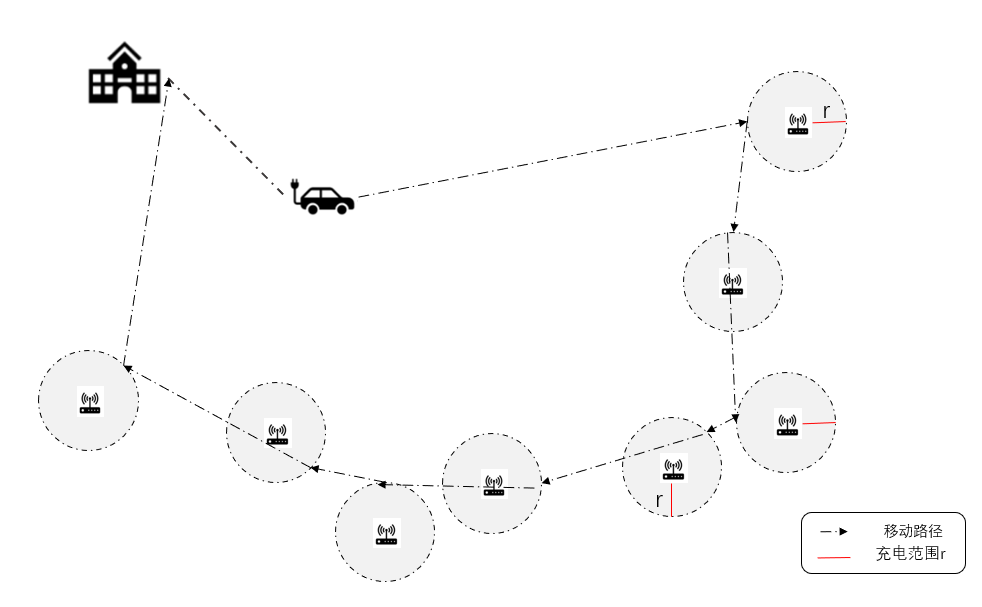
\includegraphics[width=\textwidth]{figures/bufu.png}
			\caption{充电区域不重叠时充电路线示意图}\label{asffa}
		\end{figure}
		图中传感器图形外围的虚线圆框表示对应传感器的可被充电范围,显然该情况下可充电区域不会发生,即当MC行驶至圆框内部或边界上时,即可停顿并对应传感器进行无线充电。显然,该情况下的最短路径任然为首尾相连的折线段,且停顿点数量任然等于传感器的数量,即MC的充电路线任可表示为二维有限序列如下
		\begin{gather}
		P=[ p_{1},\cdots,p_{i},\cdots,p_{29} ] ,
		\end{gather}
		其中$p_{i}(x_i,y_i)$表示MC进行充电操作时的停留点位置坐标,其必须满足充电距离约束,且每个传感器的可充电范围内至少停留了一个MC,即
		\begin{gather}
		\forall i\in[1,29]:   \underset{p_j\in P}{min}\left \{ d(s_i,p_j) \right \}\leqslant R,
		\end{gather}
	且MC在各个停留点处最多对同一传感器充电,且不会在多个停留点对同一个传感器充电,即
		\begin{gather}
		\forall i,j\in[1,29], i\neq j:  \underset{s\in S}{argmin}\left \{ d(p_i,s) \right \} \neq \underset{s\in S}{argmin}\left \{ d(p_j,s) \right \},
		\end{gather}
		其中$\underset{s\in S}{argmin}\left \{ d(p_i,s) \right \}$表示距离停留点$p_i$最近的传感器坐标 ,即表示任意两个停留点的充电目标都互不相同。且所有传感器都需要被充电,即
		\begin{gather}
		\bigcup_{i=1}^{29} \underset{s\in S}{argmin}\left \{ d(p_i,s) \right \}=S
		\end{gather}
			其中$S$表示全部传感器坐标的集合,即表示所有停留点的充电目标的集合包含了所有的传感器。目标函数仍为MC充电路线的总路程,即
		\begin{gather*}
		L(P)=d(p_0,p_{1})+d(p_0,p_{29})+\sum_{i=1}^{28}d(p_i,p_{i+1}) ,
		\end{gather*}
		即整体模型可表示为
		\begin{gather}
		min L(P) ,\\
	s.t.	\left\{\begin{matrix}1\leqslant i \leqslant 29 ,i\in Z
	\\0<R<\frac{1}{2}\underset{1\leqslant i\leqslant 29,1\leqslant j\leqslant 29,i\neq j}{max\left \{ d(s_i,s_j) \right \}},
		\\ 	\forall i\in[1,29]:   \underset{p_j\in P}{min}\left \{ d(s_i,p_j) \right \}\leqslant R,
		\\\bigcup_{i=1}^{29} \underset{s\in S}{argmin}\left \{ d(p_i,s) \right \}=S,
		\\\forall i,j\in[1,29], i\neq j:  \underset{s\in S}{argmin}\left \{ d(p_i,s) \right \} \neq \underset{s\in S}{argmin}\left \{ d(p_j,s) \right \}.
		\end{matrix}\right.
		\end{gather}
		
		当充电有效距离$R$较大,使得多个传感器的可充电范围发生重叠时,即$R$满足
		\begin{gather}
		R\geqslant \frac{1}{2}\underset{1\leqslant i\leqslant 29,1\leqslant j\leqslant 29,i\neq j}{max\left \{ d(s_i,s_j) \right \}}.
		\end{gather}
		此时充电路线大致可由图~\ref{ngf}~表示
		\begin{figure}[H]
			\centering
			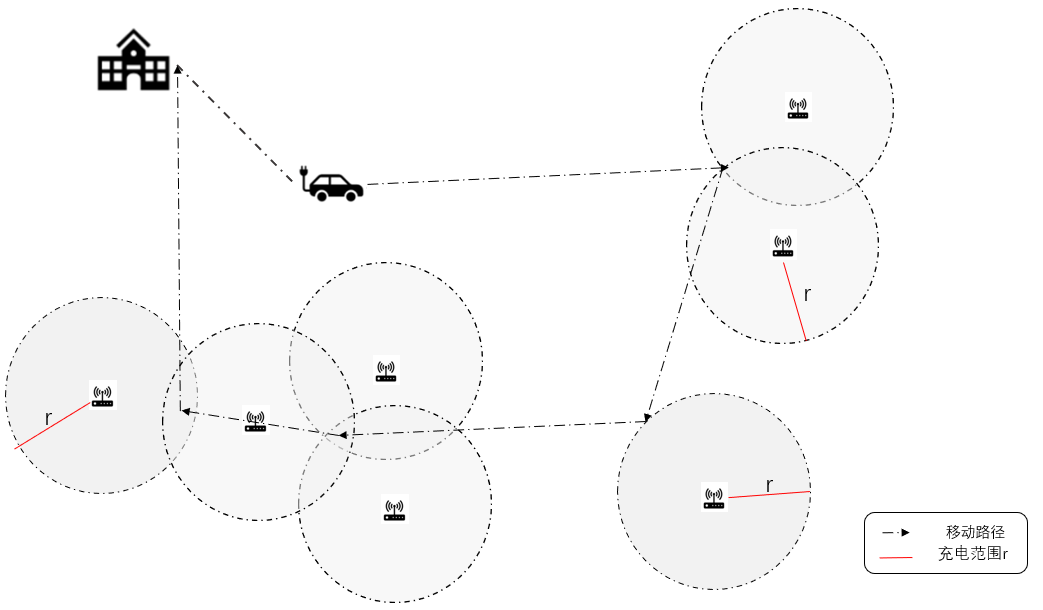
\includegraphics[width=\textwidth]{figures/fugai.png}
			\caption{充电区域重叠时充电路线示意图}\label{ngf}
		\end{figure}
	    如图所示,当可充电区域相互重叠时,我们使得停留点落在重叠区域内,即使得MC可同时对多个目标传感器进行充电。显然在此规则下,若有$k$个传感器的可充电区域发生重叠,则对应的停留点数量将变为$30-k$个,即充电路线可表示为
	    \begin{gather}
	    P_k=[ p_{1},\cdots,p_{i},\cdots,p_{30-k} ] ,
	    \end{gather}
	    目标函数仍可表示为MC充电路线的总路程,即
	    \begin{gather}
	    L(P_k)=d(p_0,p_{1})+d(p_0,p_{30-k})+\sum_{i=1}^{30-k}d(p_i,p_{i+1}) ,
	    \end{gather}
	    每个传感器的可充电范围内至少存在一个MC停留点,即
	    \begin{gather}
	    \forall s_i\in S:   \underset{p_j\in P_k}{min}\left \{ d(s_i,p_j) \right \}\leqslant R,
	    \end{gather}
	    即整体模型可表示为
	    \begin{gather}
	    min L(P_k) ,\\
	    s.t.	\left\{\begin{matrix}1\leqslant i \leqslant 29 ,i\in Z
	    \\R\geqslant \frac{1}{2}\underset{1\leqslant i\leqslant 29,1\leqslant j\leqslant 29,i\neq j}{max\left \{ d(s_i,s_j) \right \}},
	    \\ 	\forall s_i\in S:   \underset{p_j\in P_k}{min}\left \{ d(s_i,p_j) \right \}\leqslant R.
	    \end{matrix}\right.
	    \end{gather}
		\subsection{模型的求解}
		本文分别针对$R=0$、$0<R<\frac{\alpha }{2}$与$R\geqslant\frac{\alpha }{2} (\alpha =\underset{1\leqslant i\leqslant 29,1\leqslant j\leqslant 29,i\neq j}{max\left \{ d(s_i,s_j) \right \}}) $
		三种不同情况进行优化求解。当$R=0$时问题为传统TSP问题,本组设计生命遗传算法(LGA)进行优化求解。当$0<R<\frac{\alpha }{2}$时,在生命遗传算法的编码基础上,将随机梯度下降算法嵌入适应度求解过程以优化求解最佳充电路线。当$R\geqslant\frac{\alpha }{2}$时,在合并重叠区域的编码位置后,仍使用内嵌随机梯度下降的生命遗传算法对充电路线进行优化求解。
		
		\subsubsection{生命遗传算法}
		本文设计生命遗传算法,在遗传算法的基础上加入生命值衰减与个体死亡的过程以防止算法陷入局部最优解且抑制早熟,此时每个编码个体将包括三个部分如图~\ref{saf}~所示
		\begin{figure}[H]
			\centering
			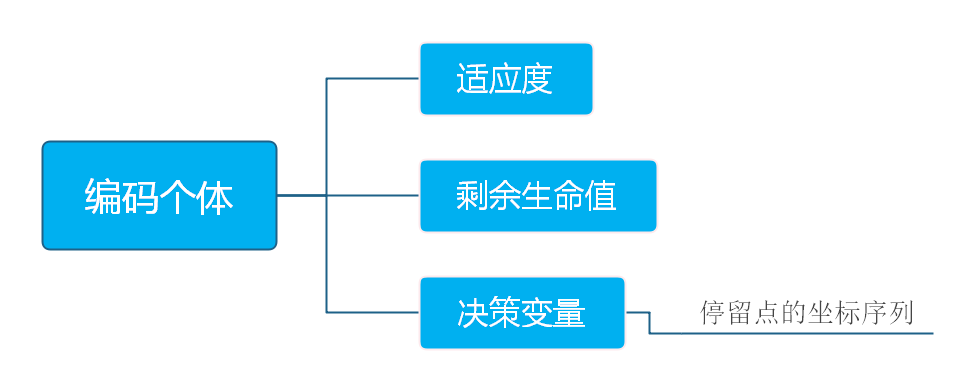
\includegraphics[width=\textwidth]{figures/lga.png}
			\caption{生命遗传算法编码个体组成}\label{saf}
		\end{figure}
		
		图~\ref{saf}~中决策变量为充电路线的整数编码,适应度即为该编码个体的决策变量对应的目标函数,剩余生命值是一个递减的整数变量。
		 \paragraph{初始化编码}
		对于表示为二维有限序列的遍历路径$P$,对其进行整数编码为
		\begin{gather*}
		A_n=[a_{n1},a_{n2},\cdots,a_{ni},\cdots,a_{n19}], \\
		1\leqslant a_i \leqslant 29 ,i\in Z ;\forall i, \neq j:p_i \neq p_j 
		\end{gather*}
		
		定义$A_n$为解序列$P_{n}$的整数编码,其中$a_{ni}$表式对传感器的访问顺序,例如 $a_{ni}=7$表示第$i$次访问7号仓库。即随机生成初始解集$\left \{A_n\right \}_0$其中$n=1,2,\cdots,w$, w为的种群容量。
		
		\paragraph{交叉}
		在原染色解集 $\left \{ A_n \right \}$中的染色体按照随机顺序配对,本文采用顺序交叉生成子代解。假定选取的交叉个体为$A_1$和$A_2$    ,其操作示意图如图~\ref{gbf}~所示
		\begin{figure}[H]
			\centering
			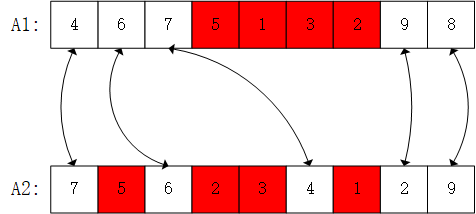
\includegraphics[width=\textwidth]{figures/cross.png}
			\caption{顺序交叉}\label{gbf}
		\end{figure}
		
		即首先选择$A1$中的一段染色体编码作为保留基因,即为图中的红色基因块部分,之后交换$A_1$与$A_2$的非保留基因段即可得到交叉子代$H_1$与$H_2$。再选取交叉个体时采用混合分组的方法,将父代均匀混合后选取所有编号为奇数的个体,与其相邻对应编号为偶数的个体,通过两种交叉方式产生交叉子代集合$\left \{ H_n \right \}$。
	     
		
		
		\paragraph{变异}
		鉴于序列式染色体的特殊性,为了在变异阶段内尽可能不破坏原有的基因段,采取改良圈算法的思路进行变异操作。即在染色体$A$中随机选取$a_{i}$与$a_{j}(1\leqslant i<j\leqslant j )$,颠倒$a_{ni}$与$a_{nj}$间顺序的顺序,即:
		\begin{gather}
		M=[a_{1},\cdots,a_{i},a_{j-1},a_{j-2},\cdots,a_{i+1},a_{i},\cdots,a_{19}]
		\end{gather}
		$M$为染色体$A$对应的变异染色体,对于每个染色体$A_n$,都设定相同的变异概率$\gamma$去执行上述的变异操作,即可产生变异子代集合产生交叉子代集合$\left \{ M_n \right \}$。 
		\paragraph{赌轮选择}
		将第g代的染色体与其交叉和变异产生的子代并入同一解集$G_g=\left \{A,H,M\right \}$。$k$表示原解集$A$,交叉解集$H$和变异解集$M$中解的数量之和,即为$G_g$中的解的数目。每次选择中,$G_g$第$i$个解$G_g(i)$被选择进入下一代的概率为
		\begin{gather}
		P(G_{g}(i))=\frac{f(G_{g}(i))}{\sum_{j=1}^{k}f(G_{g}(j))},
		\end{gather}
		$f(G_{g}(i))$为$G_{g}(i)$对应的目标函数值,即为$G_{g}(i)$对应的适应度。即在$G_g$做$w$次选择,将被选中个体放入下一代个体$\left \{A_n  \right \}_{g+1}$
		\paragraph{生命衰减}
		在每个染色体$\left \{A_n  \right \}_{g+1}$生成时设置其初始生命值为正整数$H$,即令
	\begin{gather}
	Hp(A_n)=H,
	\end{gather}
	将通过赌轮选择生成的染色体集合 $\left \{A_n  \right \}_{g+1}$,依照其适应度函数
	$f(A_n)$进行升序排列。定义其前$p$个个体为优质个体,不对其生命值经行衰减操作。对于后$w-p$个个体执行生命衰减操作。即使
		\begin{gather}
		Hp(A_n)=Hp(A_n)-1,n=p,p+1,\cdots,w.
		\end{gather}
    当个体$A_n$的剩余生命值归零,即$Hp(A_n)=0$时,我们将剔除个体$A_n$并随机生成一个新解取代其位置。
	\subsubsection{随机梯度下降}	
    	 当R>0时,本节采用随机梯度下降(Stochastic Gradient Descent, SGD)对目标函数$L(P_k)$进行寻优,即:
    	 	    \begin{gather}
    	 \begin{matrix}
    	 L(P,\Theta)=d(p_0,p_{1},\theta_0)+d(p_0,p_{30-k},\theta_{30})+\sum_{i=1}^{30-k}d(p_i,p_{i+1},\theta_{i}) ,\\ 
    	 \bigtriangledown  L(P,\Theta)= \frac{1}{m}\sum_{j=1}^{m}\bigtriangledown L(p_k,\theta_{i}),
    	 \end{matrix}
    	 \end{gather}
    	 其中$P$为中心位置向量,$\Theta$为参数方程圆周上的角度,$d(p_i,p_{i+1})$表示点$p_i$到点$p_{i+1}$的直线距离。对于任意更新$\Theta$可用伪代码描述:
    	 
    	   	\begin{algorithm}[H]
    	 	\caption{Procedure of Stochastic Gradient Descent}
    	 	\setstretch{.8}  %设置表的行间距
    	 	\LinesNumbered
    	 	\KwIn{
    	 		Number of centers: 中心位置$P$, 角度$\Theta$, 学习率$\eta$
    	 	}
    	 	\KwOut{Centers: 更新后$\Theta$}
    	 	\textbf{Initialize} $\Theta \leftarrow 0$ \newline
    	 	 	\While{True}{
     	 	
      	}
    	 	\Return {$\Theta$ }
    	 \end{algorithm}

		
    \subsection{实验结果及分析}
        对于有线充电设备,即$R=0$时,求得的最短路径如图\ref{sssssssssss}所示:
        \begin{figure}[H]
        	\centering
        	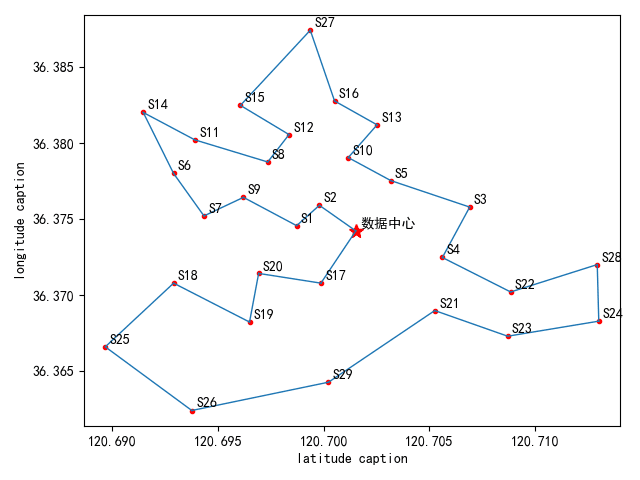
\includegraphics[width=.8\textwidth]{figures/w1.png}
        	\caption{充电半径$R=0$时移动规划路径}\label{sssssssssss}
        \end{figure}
       其充电设备规划路线为[0,2,1,9,7,6,14,11,8,12,15,27,16,13,10,5,3,4,22,28,24,23,21,\\29,26,25,18,19,20,17,0],总距离为$11482.80289m$。
        
        对于无线充电设备,求得$R=88.53m$时为临界条件,即当$0<R<88.53m$每个MC在任意位置最多同时给一个传感器充电;当$R>88.53m$时等同时对多个传感器充电。其移动规划路径分别如下图所示:
        \begin{figure}[H]
        	\centering
        	\subfigure[充电半径$0<R<88.53m$时移动规划路径]{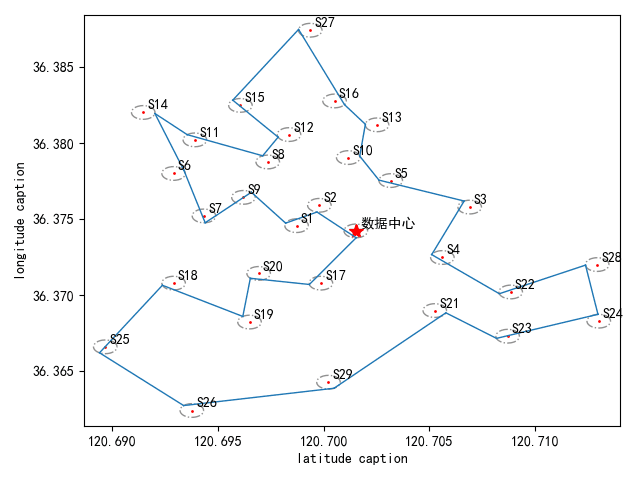
\includegraphics[height=6.5cm,width=7.5cm]{w2.png}}
        	\subfigure[充电半径$R>88.53m$时移动规划路径]{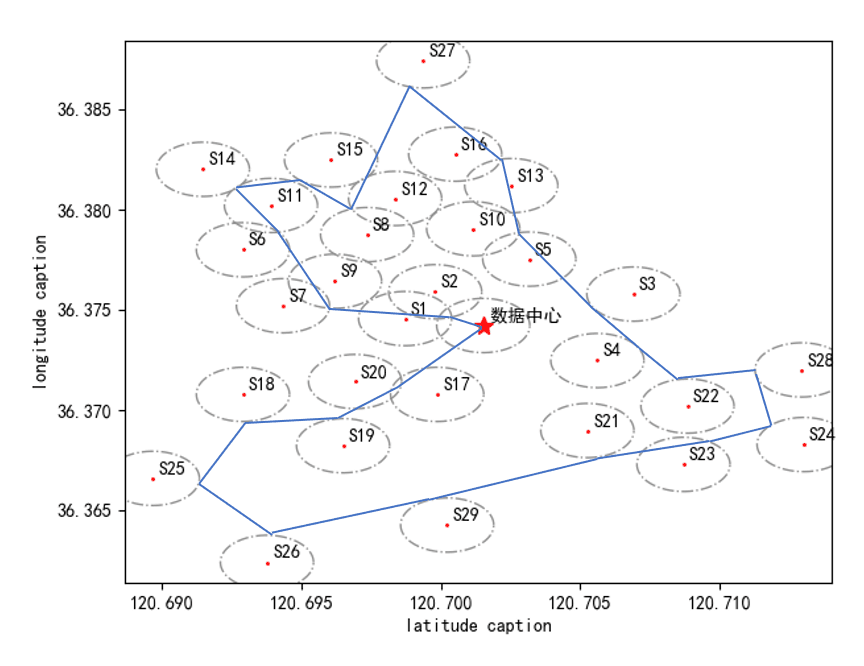
\includegraphics[height=6.5cm,width=7.5cm]{w3.png}}
        	\caption{无线充电设备移动规划路径}
        	\label{ssw}
        \end{figure}
    
    取$R=50m$,求得总距离为$11151.7684m$,其最优路线为 [0,2,1,9,7,6,14,11,8,12,15,27,16,\\13,10,5,3,4,22,28,24,23,21,29,26,25,18,19,20,17];取$R=100m$,求得总距离为$9251.6418m$,移动规划路径见图\ref{ssw}。其生命遗传算法的算法收敛图如图所示:
        \begin{figure}[H]
	\centering
	\subfigure[充电半径$0\leq R<88.53m$时算法收敛图]{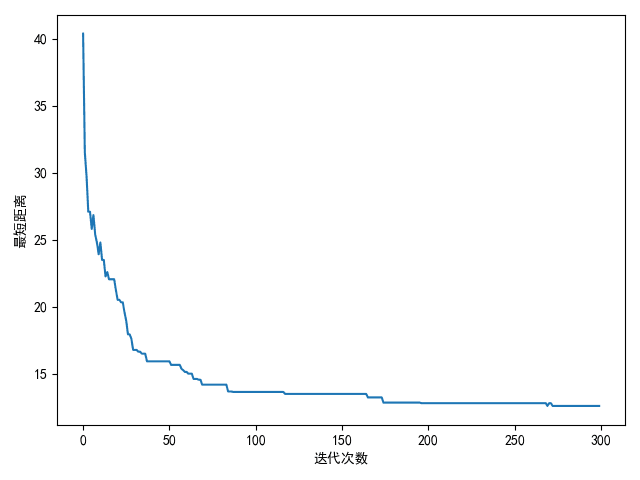
\includegraphics[height=6.5cm,width=7.5cm]{w11.png}}
	\subfigure[充电半径$R>88.53m$时算法收敛图]{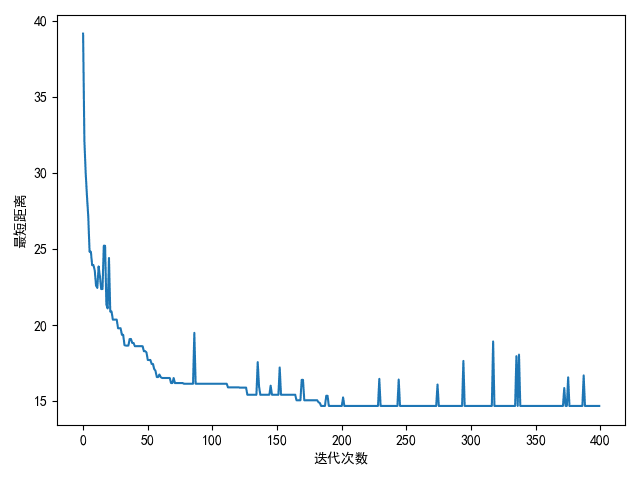
\includegraphics[height=6.5cm,width=7.5cm]{w22.png}}
	\caption{生命遗传算法收敛图}
		\end{figure}
	    由算法收敛图可知算法收敛速度较快,算法复杂度远低于遍历求解。当半径R取较小时早熟问题解决的较好,全局搜素能力较强;当R取值大于临界条件时采用随机梯度下降后收敛会出现振荡现象,但仍能搜索到局部最优解。
	
	\subsection{灵敏度分析}
	????????????????????????????????????????R越大,损失越小
	
	    \begin{figure}[H]
		\centering
		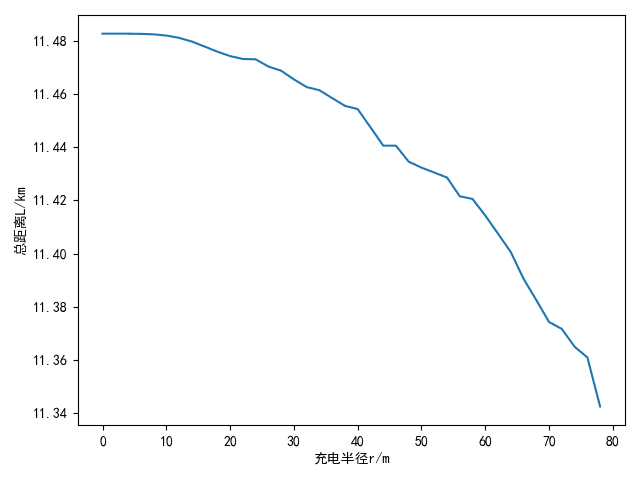
\includegraphics[width=.8\textwidth]{figures/ssss.png}
		\caption{充电半径R与移动规划路径之间的关系}\label{ssssssssssssss}
		\end{figure}
    

  
	\section{问题二模型的建立与求解}
		\subsection{问题描述与分析}

			问题二要求在问题一求得最优充电路线的基础上,给出传感器最小电池容量分布。考虑到固定周期为$T$的遍历充电模型[文献10]中能量得失分别与时间成正比,本节将充电周期划分为驻留期和移动期。一个周期内,对任意一个传感器,移动期和所有驻留期都以已知恒定速率耗电,仅在该传感器停驻的时期内以已知恒定速率充电。极限情况下,传感器能量消耗与补给的供需平衡对应传感器正常工作时的最小容量。分析能量得失去向和划分周期后,建立极限情况下的能量流动方程组,可知该模型是单值定解问题。求解方程组,可以求得传感器停留时间分布,推导停留时间和传感器电池容量的线性关系,可以获取最小能耗对应的传感器最小电池容量分布。
			其思维流程图如图~\ref{lssssct}~所示:
			
			\begin{figure}[H]
				\centering
				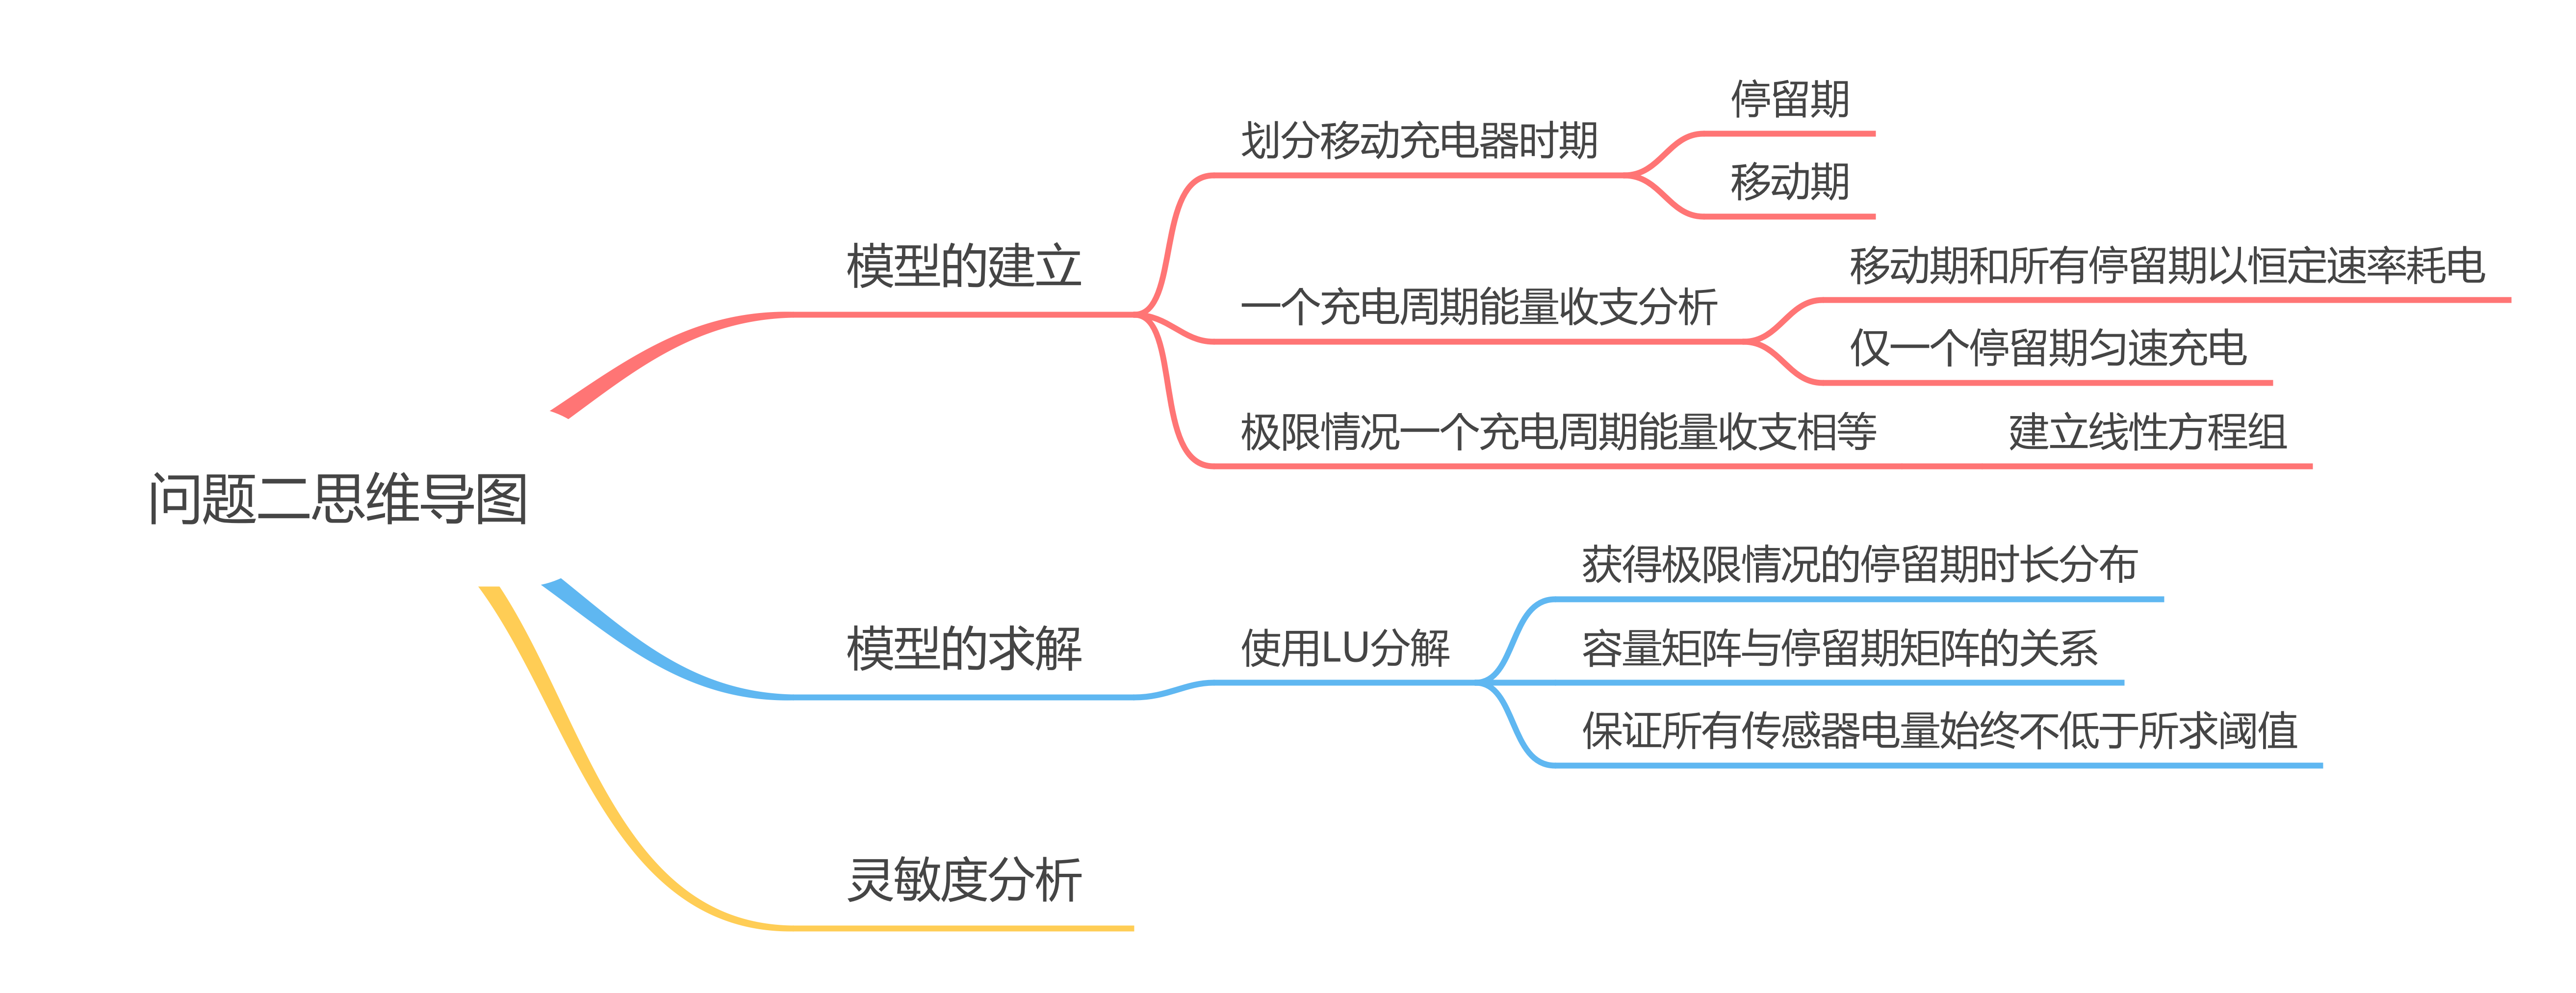
\includegraphics[width=\textwidth]{figures/222222.png}
				\caption{问题二思维流程图}\label{ssssct}
			\end{figure}
		
		\subsection{模型的建立}
			\textbf{这个地方可以细化一下}。。。。。。
			
			周期为$T$的遍历充电模型中,移动充电器循环遍历预先规划的路径,在预定区域向传感器充电。本节将充电周期$T$划分为驻留期$T_{park}$和移动期$T_{traverse}$,驻留期$T_{park}$移动充电器已经进入并静止于传感器强耦合磁共振圆域,完成移动充电器向目标传感器匀速充电的过程;移动期$T_{traverse}$,移动充电器匀速移动,移动充电器停止供电。基于模型假设,不考虑驻留期和移动期之间的时间间隔。根据能量得失去向和划分周期的关系,可列出无线可充电传感器网络正常工作时的能量流动表达式:
			\begin{gather}\label{ssssssss}
			v_{consume}\cdot (T_{traverse}+\sum_{i} T_{park}^i)\leq v_{supply}\cdot T_{park}^i.
			\end{gather}
			式\ref{ssssssss}左端和右端分别用能量流动速度与能量传递时间的乘积表示耗能和供能值。
			
			可知当所有传感器按最小电池容量分布时,传感器从移动充电器获得能量与自身消耗能量相等,即是无线可充电传感器网络正常工作的极限情况。结合已知的相关数据,对每个传感器$s_i$,有关于移动充电器在传感器$s_i$处停留时间$t_i$的$n$元线性方程组:
			\begin{gather}
			c_{j} \cdot (L/v+\sum_{i=1}^{n}t_i)=r \cdot t_j (j=1,2,...,n),
			\end{gather}
			其中,$n$是传感器数目,$L$是问题一解得最小能量消耗对应的总里程,$v$是移动充电器的移动速度,$c_{j}$是第$j$个传感器已知的能量消耗速率,$r$是充电速率。式$(1)$左右分别代表一个充电周期内消耗和补给的电量,满足传感器能量消耗与补给的供需平衡。
			
			求解这个线性方程组,可得移动充电器在所有传感器的停留时间$t_i(i=1,2,...,n)$,即驻留期分布。为了满足使用要求,传感器电量必须始终大于阈值$f$,同时保证所有传感器电量不小于$f$的使用要求。一个周期$T$内,传感器电池容量$T{threshold}$不低于驻留期$T_{park}$补充的能量$r \cdot T_{park}$,则无线可充电传感器网络正常工作时电量分布与驻留期的线性关系可表示为:
			\begin{gather}
			\left\{\begin{matrix}
			v_1\geq f+r\cdot t_1\\ 
			v_2\geq f+r\cdot t_2\\ 
			\vdots \\ 
			v_n \geq f+r\cdot t_n
			\end{matrix}\right.,
			\end{gather}
			极限情况取等号,即传感器电池容量矩阵$\bm {V_{threshold}}$与驻留期矩阵$\bm {T_{threshold}}$关系为
			\begin{gather}
			\bm{V_{threshold}}=\bm{F}+r\cdot \bm{T_{threshold}},
			\end{gather}
			其中,$\bm F$是元素全为传感器电量阈值$f$的规格为$n \times 1$的列向量,$\bm{T_{threshold}}$是$t_1,t_2,...,t_{n}$按顺序构成的规格为$n\times 1$的列向量,$r$是充电速率。
    		
    		

		
		
		\subsection{模型的求解}
		\textbf{再完善一下内容。。。}
		对于单值定解问题,使用矩阵分解方法分解求解。目前矩阵分解方法主要有$LU$分解、$LUP$分解、谱分解、$Cholesky$分解、$QR$分解、奇异值分解等方法。考虑到问题二目标矩阵$A$具有阶数高、是$n$阶方阵、$A$的前$rank(A)$阶顺序主子式不为$0$等特征,可以看出是一阶线性方程组,考虑到左边方阵直接求逆计算复杂度较大,故化简后使用$LU$分解法求解。$LU$分解的最大计算复杂度是$O(n^3)$,具有无需判定矩阵是否正定,浮点数操作总量都在$O(n^2)$(双重循环)等优点。
		
		化简$(1)$式,得矩阵方程
		\begin{gather}
		\bm A \cdot \bm{T_{threshold}}=-L/v \cdot \bm b,
		\end{gather}
		或表示为
		\begin{gather}
		\begin{bmatrix}
		1-\frac{r}{c_1} & 1 & ... & 1 \\ 
		1 & 1-\frac{r}{c_2} & ... & 1\\ 
		\vdots  & \vdots & \ddots  & \vdots \\ 
		1 & 1 & ... & 1-\frac{r}{c_n}
		\end{bmatrix}\begin{bmatrix}
		t_1\\ t_2\\ \vdots\\ t_n
		\end{bmatrix}=-\frac{L}{v}
		\begin{bmatrix}
		1/c_1\\ 1/c_2\\ \vdots\\ 1/c_n
		\end{bmatrix},
		\end{gather}
		其中$t_i(i=1,2,...,n)$是极限情况时,无线充电器在传感器$s_i$处的停留时间,$c_i(i=1,2,...,n)$表示传感器$s_i$能量消耗速率,$r$是固定的充电速率。
		
		根据$LU$分解原理,有
		\begin{gather}
		\bm{Ly}=-L/v\cdot \bm b,\\s.t.
		\left\{\begin{matrix}
		y_1=b_1
		\\ 
		y_k=b_k-\sum_{j=1}^{k-1}l_{kj}y_j
		\end{matrix}\right.,k=2,3,...,n,\\
		\bm{UT_{threshold}}=-L/v \cdot \bm{L^{-1} b},\\s.t.
		\left\{\begin{matrix}
		y_n=y_n/u_{nn}
		\\ 
		t_k=(y_k-\sum_{j=k+1}^{n}u_{u_{kj}t_j})/u_{kk}
		\end{matrix}\right.,k=n-1,n-2,...1.
		\end{gather}
		结果如表\ref{biao2}所示:
		\begin{table}[H]
			\setstretch{1}  %设置表的行间距
			\centering		
			\caption{传感器电池最小容量分布}\label{biao2}
			\begin{tabular}{cccc}
				\toprule[2pt]
				\multicolumn{1}{m{2.5cm}}{\centering 传感器序号}
				& \multicolumn{1}{m{4.5cm}}{\centering 传感器最小电池容量}& \multicolumn{1}{m{2.5cm}}{\centering 传感器序号}& \multicolumn{1}{m{4.5cm}}{\centering 传感器最小电池容量}
				\\
				\midrule[1pt]
				2 &   5001.24202643 & 3&4801.81519446\\ 
				1&   5533.04691166& 4&5023.40056331\\ 
				9&   4801.81519446& 22&5466.57130101\\ 
				7 &   5023.40056331& 28&5023.40056331\\ 
				6 &   4602.3883625 & 24&4801.81519446\\ 
				14&   4801.81519446& 23&4580.22982561\\ 
				11 &  5222.82739527& 21&5023.40056331\\ 
				8&  4823.97373135& 29&5466.57130101\\ 
				12&   4801.81519446& 26&4580.22982561\\ 
				15 &  5023.40056331& 25&5023.40056331\\ 
				27&  4801.81519446& 18&4757.49812069\\ 
				16&  5444.41276412& 19&4602.3883625 \\ 
				13 &  5244.98593216& 20&5222.82739527\\ 
				10 &  4801.81519446& 17&5001.24202643\\ 
				5 &  4646.70543627& &\\
				\bottomrule[2pt]	
			\end{tabular}
		\end{table}
		
		由表\ref{biao2}可知
		
        \subsection{灵敏度分析}

		改变移动充电器的移动速度、充电速率、能量圆域半径和传感器电量阈值,观察$30$个传感器电池容量的变化情况。
		
	\begin{figure}[H]
		\centering
		\subfigure[最大25km,升级20个水管]{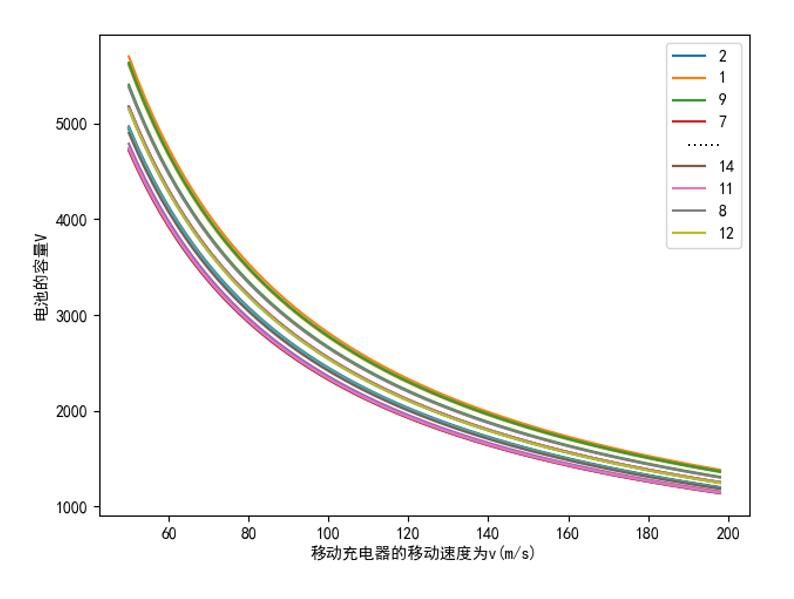
\includegraphics[height=6.5cm,width=7.5cm]{2333v.jpg}}
		\subfigure[最大30km,升级11个水管]{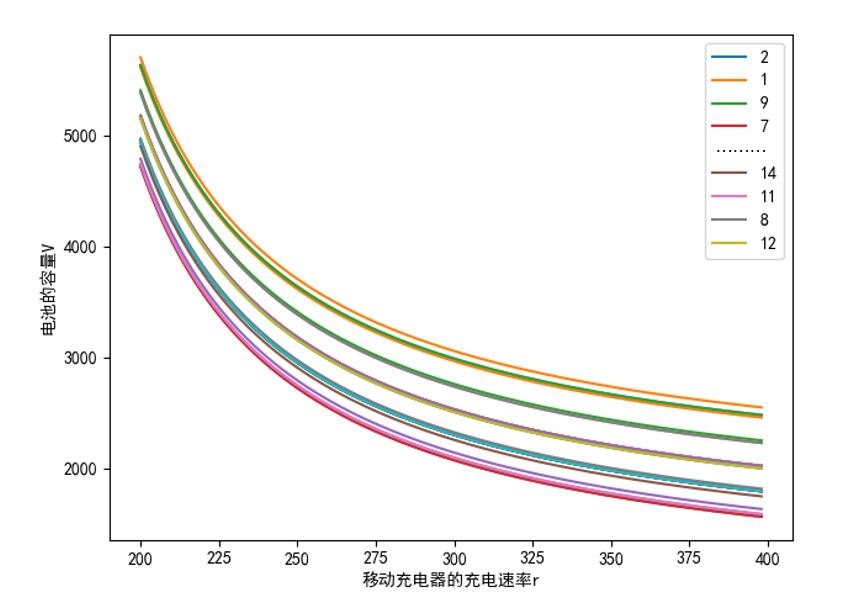
\includegraphics[height=6.5cm,width=7.5cm]{2333r.jpg}}
	\end{figure}	
	\begin{figure}[H]
		\centering
		\subfigure[最大35km,升级7个水管]{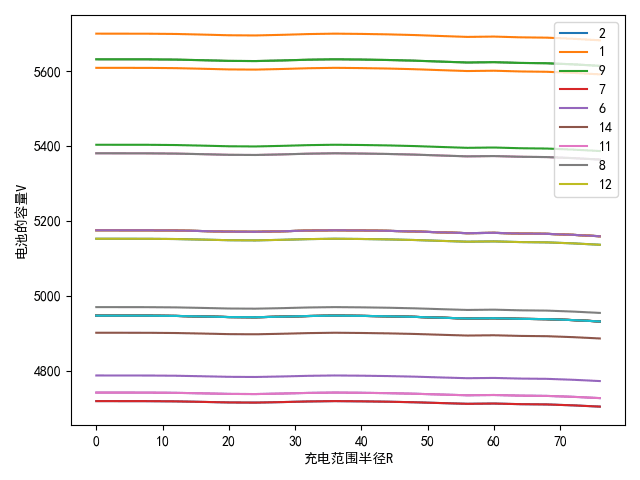
\includegraphics[height=6.5cm,width=7.5cm]{2333R.png}}
		\subfigure[最大40km,升级1个水管]{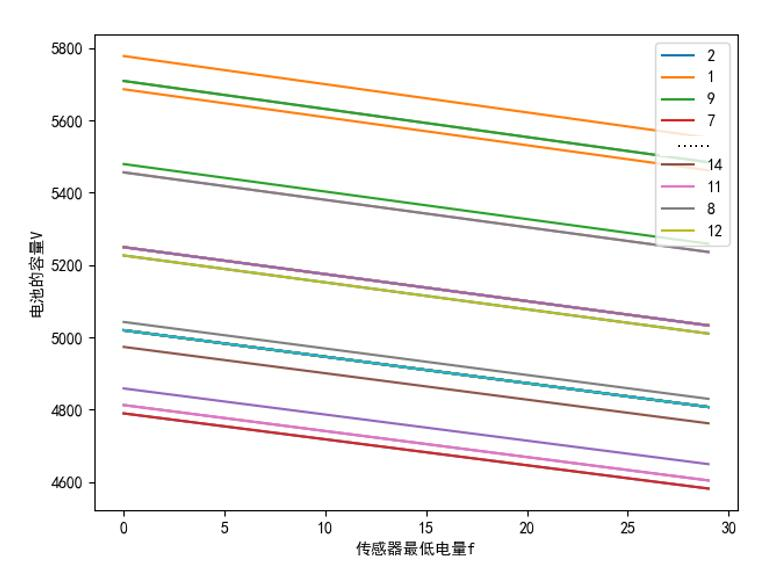
\includegraphics[height=6.5cm,width=7.5cm]{2333f.jpg}}
		\caption{不同二级管道铺设最大代价}
		\label{mgh}
	\end{figure}
		根据图\ref{mgh}分析可知,$0$到$70m$范围内能量圆域半径$R$变化对传感器电池容量分布几乎无影响,而移动充电器的移动速度$v$、充电速率$r$和传感器电量阈值$f$的增大会引起所有传感器电池容量下降,其中传感器电量阈值$f$增大引起的电池容量降低效应是线性的,这是由于移动充电器充电速率$r$远大于给定的传感器能量消耗速率$c_j(j=1,2,...,29)$,使得式(5)对角元系数为负值,驻留期时间$t_i(i=1,2,...,29)$线性减少效应大于传感器电量阈值$f$的增大效应。
		



    \section{问题三模型的建立与求解}
  		\subsection{结果分析}
  
  	\section{灵敏度分析}
 
  	\section{模型的评价}
		\subsection{模型的优点}
			\begin{itemize}                                             
			\item [(1)]
			\item [(2)] 	
			\end{itemize}
		\subsection{模型的缺点}

  		\subsection{模型改进}

  
  
 
	\newpage	%换页符
	%%参考文献
	%\begin{thebibliography}{9}%宽度9
	% \setlength{\itemsep}{-2mm}
	\nocite{*}		%排版未引用的参考文献
	\begin{thebibliography}{9}%宽度9
		\bibitem{1}Othman M F, Shazali K. Wireless sensor network applications: A study in environment monitoring system[J]. Procedia Engineering, 2015, 41: 1204-1210.
		\bibitem{2}Borges L M, Velez F J, Lebres A S. Survey on the characterization and classification of wireless sensor network applications[J]. IEEE Communications Surveys \& Tutorials, 2014, 16(4): 1860-1890.
		\bibitem{3}Xie L, Shi Y, Hou Y T, et al. Making sensor networks immortal: An energy-renewal approach with wireless power transfer[J]. IEEE/ACM Transactions on networking, 2012, 20(6): 1748-1761.
		\bibitem{4}Tarng W, Ou K L, Huang K J, et al. Applying cluster merging and dynamic routing mechanisms to extend the lifetime of wireless sensor networks[J]. International Journal of Communication Networks and Information Security, 2011, 3(1): 8.
		\bibitem{5}曲立军, 党鑫, 武继刚. 无线传感器网络中的充电调度算法[J]. 计算机与数字工程, 2017, 45(2): 319-326.
		\bibitem{6}Butler Z, Rus D. Controlling mobile sensors for monitoring events with coverage constraints[C]//IEEE International Conference on Robotics and Automation, 2004. Proceedings. ICRA'04. 2004. IEEE, 2004, 2: 1568-1573.
		\bibitem{7}Yao W, Li M, Wu M Y. Inductive charging with multiple charger nodes in wireless sensor networks[C]//Asia-Pacific Web Conference. Springer, Berlin, Heidelberg, 2006: 262-270.
	
	\end{thebibliography}

	\newpage
	%附录
	\appendix %%附录
	\section{数据可视化的实现}
		\subsection*{第一问画图--python源代码}
			\begin{lstlisting}[language=python]
			
			\end{lstlisting}
			
		\subsection*{第二问画图--python源代码}
			\lstinputlisting[language={python},numbers=left,numberstyle=\tiny,
			rulesepcolor=\color{red!20!green!20!blue!20},  
			keywordstyle=\color{blue!70!black},  
			commentstyle=\color{blue!90!},  
			basicstyle=\ttfamily] {./code/demo.py}

\end{document}